\chapter{Contexte du projet}
%\markboth{Chapitre 1 }{Contexte du projet} %pour afficher l'entete
%\addcontentsline{toc}{chapter}{Chapitre 1 : Contexte du projet}


\section{Introduction}
Le premier chapitre de ce rapport présente l'organisme d'accueil ainsi que le projet de déploiement de l'infrastructure IT et SI d'une entreprise et l'intégration d'objet connectés au réseau. \\

Nous commençons  par une présentation de l'entreprise et de ses activités, ainsi que de ses objectifs en matière de technologies connectées. Ensuite, nous expliquons le contexte dans lequel s'inscrit ce projet, en évoquant les enjeux et les besoins auxquels il répond.\\

Enfin, nous présentons  les parties prenantes impliquées dans ce projet, ainsi que leurs rôles respectifs dans sa réalisation. Ce premier chapitre permettra ainsi de poser les bases nécessaires pour la compréhension du projet et de ses enjeux.\\



Le premier chapitre de ce rapport présente l'organisme d'accueil ainsi que le projet de déploiement de l'infrastructure IT et SI d'une entreprise et l'intégration d'objet connectés au réseau. \\

 Nous commençons par une présentation de entreprise et de ses activités, ainsi que de ses objectifs en matière de technologies connectées. Ensuite, nous expliquons le contexte dans lequel s'inscrit ce projet, en évoquant les enjeux et les besoins auxquels il répond.\\
 
Enfin, nous présentons les parties prenantes impliquées dans ce projet, ainsi que leurs rôles respectifs dans sa réalisation. Ce premier chapitre permet ainsi de poser les bases nécessaires pour la compréhension du projet et de ses enjeux. \\


\section{Présentation de l'organisme d'accueil }

Dans cette section, nous abordons la présentation de l'organisme d'accueil Zeta Engineering ainsi que son domaine d'activités.

\subsection{Organisme d'accueil}


Notre stage de projet de Mémoire De Mastère a été réalisé chez Zeta Engineering, un bureau d'étude multifonction appartenant au groupe Agexis \cite{agexis}, qui intervient sur la zone européenne et africaine. \\

Nous avons effectué ce stage dans le cadre de l'obtention de notre diplôme de Mastère Professionnel Co-construit en Infotronique. \\

Le groupe Agexis est un bureau d'étude technique pluridisciplinaire et maître d'oeuvre du bâtiment et des infrastructures. Il est implanté en Île-de-France depuis 2015.  \\


AB Engineering, une autre filiale du groupe, est également un bureau d'étude technique pluridisciplinaire et maître d'oeuvre du bâtiment et des infrastructures, implanté en Île-de-France depuis 2011. \\


Quant à Zeta Engineering, elle est spécialisée dans le consulting et l'engineering, et se consacre principalement au conseil en communication, marketing, IT et gestion pour les entreprises, en Tunisie comme en France. Elle est basée en Tunisie depuis 2018. \\


Zeta Engineering est située à l'adresse 58 Rue de la Solidarité à Rades Méliane en Tunisie. \\


Nous avons été encadrés par une équipe de professionnels compétents et expérimentés lors de notre stage, durant lequel nous avons travaillé sur un projet passionnant dans le domaine IT. \\





\subsection{Domaines d'activités}
Zeta Engineering, en collaboration avec AGEXIS et AB Engineering, est chargée de mettre en place leur stratégie marketing pour la période 2020-2030, en déployant leur communication et leur commercialisation. \\


Ce entreprise de bureau d'étude multifonction est située en Tunisie et travaille en étroite collaboration avec Agexis. Les services proposés par Zeta Engineering sont très diversifiés et couvrent différents secteurs. \\

Zeta Engineering s'appuie sur son expertise technique et son expérience pour fournir des solutions d'ingénierie innovantes et de haute qualité, depuis la phase de conception jusqu'à la production, en passant par la simulation, la modélisation, la validation et la certification.  \\





\section{Présentation du projet}

Dans cette section, nous abordons le cadre de notre projet, ainsi que la problématique de notre projet.


\subsection{Cadre de projet}
Dans le cadre de notre projet de mémoire mastère, nous avons été accueillis au sein de Zeta Engineering. Notre mission consiste à mettre en place une infrastructure IT et SI pour relier les trois bureaux de l'entreprise, situés respectivement à Rades Habib Bourgiba, Rades Meliane et Ezzahra, via un réseau MAN.\\


\begin{table}[H]
\begin{center}
     \begin{tabular}{|c{5cm}|c{5cm}|c{5cm}|}
    \hline
	\textbf{Logo}         & \textbf{Adresse}   & \textbf{Fonctionnalité} \\
    \hline
    
	
\includegraphics[width=5cm]{Images/logo-zeta1.png} & Rades Meliane, Rue de la Solidarité  & Réservé à l'administration et Diffusion Globale  \\
	
 	\hline
 	
	\includegraphics[width=5cm]{Images/logo-Sequencia.png}   &  Rades, Rue Habib Bourgiba  &  Centre d'appel \\
	
	\hline
	
	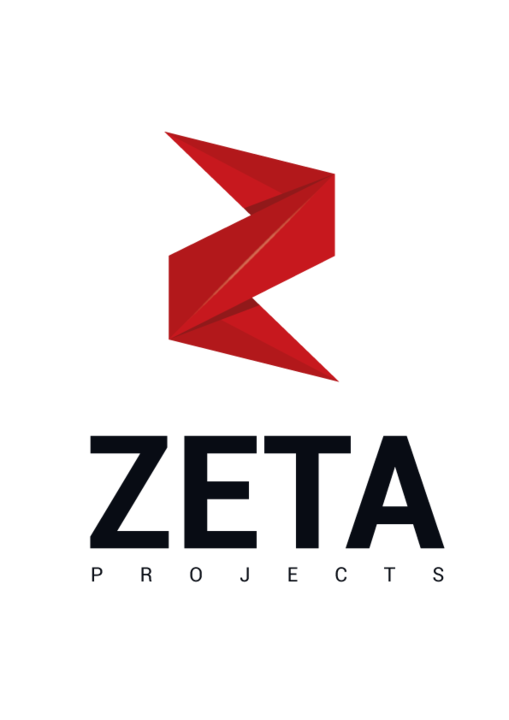
\includegraphics[width=5cm]{Images/Logo-ZetaProject.png}  & Ezzahra, Rue Habib Bourgiba    & Abrite les ingénieurs et les développeurs Informatique  \\
	
	\hline
	
     \end{tabular}
     \caption{Les nouveaux Locaux de Zeta}
     \label{1}
     \end{center}
\end{table}

Notre projet consiste également à connecter les objets tels que les machines de pointage, les thermostats, les lampes, les smartphones et les caméras de surveillance pour une utilisation plus efficace de ces ressources au sein de l'entreprise.\\

\subsection{Problématique}
L'intégration d'un système d'information avec des objets connectés représente un défi majeur pour de nombreuses entreprises qui cherchent à améliorer leur efficacité et leur compétitivité.\\

Cette transition soulève des problématiques complexes, telles que la gestion de données massives, la sécurité des systèmes, la compatibilité des technologies et la formation des employés.\\

Comment surmonter ces défis pour réussir la transition d'un système d'information traditionnel vers un système d'information intégrant des objets connectés ? Quelles sont les meilleures pratiques, les outils et les stratégies à adopter pour assurer une intégration réussie et durable ? \\

En explorant ces questions, nous mettons en évidence l'importance du déploiement efficace des infrastructures IT et SI ainsi que l'intégration réussie des objets connectés pour soutenir les activités opérationnelles des entreprises.



\section{Méthodologie de travail et planification}

Dans cette section, nous abordons la présentation d'une méthodologie, ainsi que la problématique de notre projet.


\subsection{Présentation de la méthodologie}

Dans le vaste éventail de méthodologies de gestion de projet, telles que le modèle en V, la méthodologie itérative, Scrum, et bien d'autres, nous avons choisi d'adopter le modèle en cascade pour notre projet. Aussi connue sous le nom de méthodologie en cascade, cette approche séquentielle est souvent privilégiée dans les projets de Mémoire De Mastère en raison de sa simplicité et de sa facilité de compréhension.

Le choix de la méthodologie en cascade repose sur divers facteurs spécifiques à notre projet. Tout d'abord, nous avons identifié que les besoins et les exigences du projet étaient relativement bien connus et stables dès le départ. Cette méthodologie convient parfaitement lorsque les étapes du projet peuvent être définies en amont et que les changements ne sont pas susceptibles d'être fréquents.

De plus, notre équipe avait une compréhension claire des objectifs à atteindre et de la séquence des tâches à accomplir. Cette méthode en cascade nous a fourni un cadre structuré pour aborder chaque étape de manière méthodique, permettant une planification précise et une gestion efficace des ressources. 

En somme, le modèle en cascade s'est avéré approprié pour notre projet en fournissant une structure bien définie qui a facilité la gestion des différentes phases du déploiement de l'infrastructure IT, de l'infrastructure SI et de l'intégration des objets connectés. \\


La figure \ref{Chap1.4} illustre les étapes caractéristiques de la méthodologie en cascade. Cette approche linéaire \cite{blogcasacade} et séquentielle guide le projet à travers une série d'étapes bien définies. Initiant avec l'analyse des besoins et la planification, elle progresse ensuite vers la conception, la réalisation, les tests et enfin, la phase de déploiement et de maintenance. Chaque phase est traitée de manière séparée et successive, avec des étapes claires et spécifiques à accomplir avant de passer à la suivante. Cette structure rigoureuse garantit une progression ordonnée du projet, en mettant l'accent sur la finalisation de chaque étape avant de passer à la suivante.


\begin{figure}[H]
 \centering
    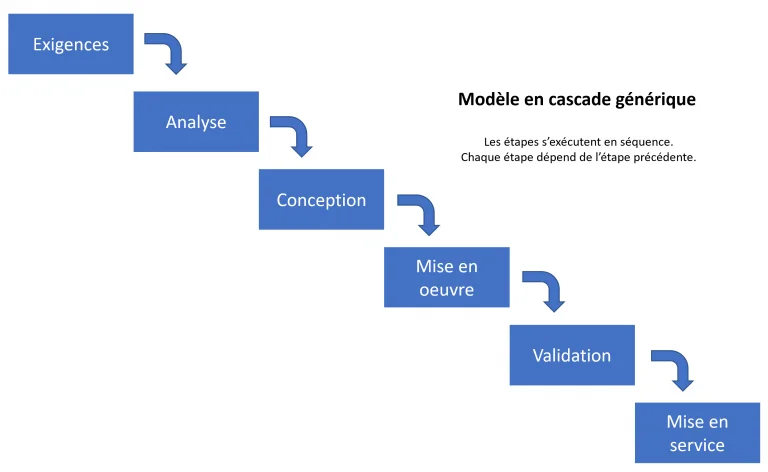
\includegraphics[width=15cm]{Images/cascade1.png}
    \caption{Méthodologie en Cascade}
    \label{Chap1.4}
\end{figure}

Le processus de la méthodologie en cascade se divise en plusieurs phases séquentielles, chacune étant une étape préalable à la suivante. Les étapes typiques incluent la définition des besoins, l'analyse, la conception, la mise en œuvre, les tests et la maintenance. \\

Dans cette méthodologie, chaque étape doit être achevée avant que la suivante puisse commencer. Les étapes ne peuvent pas être rétrogradées et doivent être effectuées dans l'ordre établi. Cela signifie que le projet doit être entièrement défini et spécifié avant que la conception ne puisse commencer, et que la conception doit être terminée avant que la mise en œuvre puisse commencer, et ainsi de suite. \\



\subsection{Choix de Cascade}
Étant donné que notre projet comporte plusieurs étapes qui dépendent de l'étape précédente, notre organisme d'accueil nous a demandé d'utiliser la méthode en cascade. Cette approche implique de terminer une phase du projet avant de passer à la suivante.\\ 


Ainsi, chaque chapitre de notre rapport se consacre à expliquer les choix matériels et logiciels adoptés, ainsi qu'à détailler l'exécution de chaque composant du projet. Cette méthodologie nous permet de travailler de manière organisée et structurée, en veillant à ce que chaque étape soit achevée de manière adéquate avant de passer à la suivante \cite{fagarasan2021agile} .\\\\\




\section{Conclusion }
En conclusion, ce premier chapitre nous a permis de présenter l'organisme d'accueil Zeta Engineering et son contexte de projet, qui consiste à ouvrir trois nouveaux bureaux à Rades, Rades Meliane et Ezzahra.\\

Nous avons également abordé la méthodologie choisie pour la gestion de ce projet, à savoir la méthode en cascade, qui nous permet de travailler de manière séquentielle en terminant chaque phase avant de passer à la suivante. Les choix matériels et logiciels pour chaque étape sont également détaillés dans les chapitres suivants afin d'assurer une bonne exécution du projet. \\


